%auto-ignore
%      this ensures the arxiv doesn't try to start TeXing here.
%!TEX root = super_lattice_models_draft.tex
%      prev line helps TeXShop do the right thing

%%%%%%%%%%%%%%%%%%%%%%%%%%%%%%%%
\section{Quasiparticle excitations and the tube category of $C_2$} \label{C2_quasiparticles}
%%%%%%%%%%%%%%%%%%%%%%%%%%%%%%%%

In this section, we identify the quasiparticle excitations 
in the $C_2$ theory.
We will discuss the quasiparticles in the theory, their fusion rules, their statistics, and the 
modular transformations of the ground states on the torus.
We will identify the excitations using a fermionic generalization of a device known as the {\it tube category}. 
We will briefly review the tube category as applied to the $C_2$ theory below; 
for a more detailed overview and for an explanation of why the fermionic version of the tube category computes the excitations, 
we refer the reader to Section \ref{more_on_tubes}, where we discuss the construction in full generality. 

For the benefit of more physically-inclined readers 
we will use the ``Hamiltonian/ground-state/excitation'' terminology 
in this section, 
even though (as discussed in the introduction) we will not define the relevant Hamiltonian until Section \ref{Super_pivotal_Hamiltonian}.
The constructions in this section all take place within the self-contained world of TQFTs defined via string nets;
the Hamiltonian/ground-state/excitation interpretation is optional.


%%%%%%%%%%%%%%%%%%%%%%%%%%%%%
\subsection{Finding the quasiparticle excitations}   \label{C2excitations}
%%%%%%%%%%%%%%%%%%%%%%%%%%%%%

We now turn to a detailed study of the tube category for $C_2$. 
The objects of $\tube(C_2)$ are given by spin circles with a finite number of marked points 
labeled by simple objects of $C_2$.
There are two spin structures on the circle: bounding (anti-periodic boundary conditions; non-vortex) and 
non-bounding (periodic boundary conditions; vortex).
Each object in $\tube(C_2)$ thus determines a choice of spin structure of the underlying circle. 

It suffices to consider only objects with at most one labeled point.
This is because any other object is isomorphic to a direct sum of objects with at most one labeled point.
Note also that an object with a point labeled by $\mathds{1}$ (the trivial object of $C_2$)
is isomorphic to the object obtained by erasing that marked point.
In particular, a circle with no marked points is isomorphic to a circle with a single point labeled by $\mathds{1}$.


Since there are two simple objects in $C_2$, 
for a fixed spin structure there are only two possible labels that can be assigned to a marked point,
\begin{align}
\underset{\mathds{1}}{\TubeBCx{B}} \quad \quad \quad \underset{\beta}{\TubeBCx{B}} \quad \quad \quad \quad \quad \quad \underset{\mathds{1}}{\TubeBCx{N}} \quad \quad \quad \underset{\beta}{\TubeBCx{N}}
\end{align}
where $B$, $N$ denote bounding and non-bounding spin structures respectively. 

Morphisms of $\tube(C_2)$ are 
defined to be cylinders (which we will draw as annuli) decorated by $C_2$ string-nets.
A given morphism $a\ra b$ is thus an annulus whose outer (inner) boundary conditions are determined by the object $a$ ($b$). 

After applying local relations (F-moves, dot-cancellations, removing trivial loops), 
an arbitrary string-net diagram on any tube can be reduced to a linear 
combination of the following diagrams:
\be
\begin{aligned}
\label{mortube}
\text{mor}(\underset{\mathds{1}}{\TubeBCx{J}} \rightarrow \underset{\mathds{1}}{\TubeBCx{J}}) &= \mathbb{C}\left[ \Fubex{\FubeXXXA}{J} ,  \Fubex{\FubesXsA}{J}, \Fubex{\FubesdXsA}{J} \right] \\
\text{mor}(\underset{\beta}{\TubeBCx{J}} \rightarrow \underset{\beta}{\TubeBCx{J}}) &= \mathbb{C}\left[   \Fubex{\FubeXssA}{J} ,  \Fubex{\FubessXA}{J}, \Fubex{\FubeXsdsA}{J} , \Fubex{\FubessdXA}{J} \right] \\
\\
\text{mor}(\underset{\mathds{1}}{\TubeBCx{B}} \rightarrow \underset{\beta}{\TubeBCx{N}}) &= 0 \quad \quad \quad \quad \text{mor}(\underset{\beta}{\TubeBCx{N}} \rightarrow \underset{\mathds{1}}{\TubeBCx{B}}) = 0
\end{aligned}
\ee
with $J =B$ for bounding spin structure, and $J =N$ for non-bounding spin structure. 
In the first row we have listed all possible tubes which take the trivial boundary condition back to itself, 
and in the second row the tubes which take the $\beta$ marked point back to itself.
Notice that all non-zero tubes for $C_2$ have the same label at the two marked points.
For general input categories this won't happen; see Sections \ref{so36} and \ref{halfesix} for examples.



Depending on the spin structure on the annulus, some of the above diagrams may be zero.
With a bounding spin structure, a fermionic dot picks up a factor of $-1$ if it moves around the annulus.
On the other hand a fermionic dot picks up a factor of $+1$ if it moves around the annulus with non-bounding spin structure.

As we said above, not every string diagram in the annulus is consistent with a given spin structure.
For example,
\begin{align}
\label{BoundingNullVector}
\Fubex{\FubesdXsA}{B}\;  = - \; \Fubex{\FubesdXsA}{B} \implies \Fubex{\FubesdXsA}{B} = 0,
\end{align}
where we have simply pulled the fermion around the non-contractible loop on the tube. 
A non-bounding tube with a horizontal $\beta$ line is also zero, since
\begin{align}
\label{non-boundingNullVector}
\Fubex{\FubesXsA}{N}\; =\; A^{-4} \Fubex{\FubesXsaA}{N} \; = A^{-4} \Fubex{\FubesXscA}{N} \; = \; -\Fubex{\FubesXsA}{N}
\end{align}
Where in the second step we have dragged one of the two fermions around the annulus.
All other tubes are nonzero for both spin structures, and so a complete basis for tubes in the bounding sector is given by
\begin{align}
 \label{atubes}
\tube^B_{\unit \rightarrow \unit} &= \mathbb{C} \left[\Fubex{\FubeXXXA}{B}  ,\Fubex{\FubesXsA}{B}\right]\\
\tube^B_{\beta \rightarrow \beta}  &=  \mathbb{C} \left[\Fubex{\FubeXssA}{B}  ,\Fubex{\FubessXA}{B},\Fubex{\FubeXsdsA}{B},\Fubex{\FubessdXA}{B}\right]
\end{align}
while a basis for the non-bounding sector is given by
\begin{align}
\label{ptubes}
\tube_{\unit \rightarrow \unit}^N &= \mathbb{C}\left[ \Fubex{\FubeXXXA}{N}  ,\Fubex{\FubesdXsA}{N} \right]\\
\tube_{\beta \rightarrow \beta}^N &= \mathbb{C}\left[ \Fubex{\FubeXssA}{N}  ,\Fubex{\FubessXA}{N} ,\Fubex{\FubeXsdsA}{N} ,\Fubex{\FubessdXA}{N}  \right]
\end{align}

The multiplication operation in the tube category is given by stacking tubes on top of one another 
and simplifying the resulting tube using local relations.  
For example, in the non-bounding sector we have
\begin{align}
\label{OddOddC2Stack}
\Fubex{\FubesdXsA}{N} \;  \cdot  \; \Fubex{\FubesdXsA}{N}  \;=\; \Fubex{\FubesddXsA}{N} \;=\; \frac{1}{d} \left(
\Fubex{\RDotTwobA}{N}
+ A^{-4} \Fubex{\RDotTwocA}{N}  \right) \; = \; 2 \Fubex{\FubeXXXA}{N}
\end{align}

Note that since the spin structures on two tubes being fused must agree on the boundary 
at which they are fused, non-bounding tubes can only be stacked on top of non-bounding tubes, 
and similarly for bounding tubes.



Relations like the ones above allow us to find the (isomorphism classes of) minimal idempotents of the tube category. 
First, we turn to an analysis of tubes with bounding spin structure. 



%%%%%%%%%%%%%%%%%%%%%%%
\subsubsection{Non-vortex spin structure}
%%%%%%%%%%%%%%%%%%%%%%%%

Let us first examine the tubes with no charge,\footnote{
We define the ``charge'' of a tube to be the label of the 
marked point of the upper boundary of the tube, so that tubes in $\tube_{a \rightarrow b}$ have charge $b$. 
This is slightly misleading however, because charge is not a good quantum number: in more general theories, 
$\tube_{a \ra b}$ will be nonzero even when $a\neq b$. 
}
that is, cylinders 
with bounding spin structures and empty boundary conditions on both their top and bottom, which are the cylinders in $\tube^B_{\unit \rightarrow \unit}$. 
We see that this algeba \eqref{atubes} has two even generators, and so as a vector space
\begin{align}
\label{C2etoe}
\tube^B_{\unit \rightarrow \unit} \cong \mathbb{C}^{2|0}
\end{align}
There is only one possible super algebra structure on $\mathbb{C}^{2|0}$; it is the sum of two trivial 1-dimensional algebras
$\End(\cc)\oplus \End(\cc)$ (or $\cc \oplus \cc$ for short, where here $\cc$ denotes a 1-dimensional 
algebra rather than a 1-dimensional vector space).
This sector therefore contains two minimal idempotents, which we will call $m_\unit$ and $m_\psi$.
Explicitly, they are 
\be
m_\unit = \frac{1}{2}\left( \Fubex{\FubeXXXA}{B} \; +\; \frac{1}{d}\Fubex{\FubesXsA}{B}\right),\qquad 
m_\psi = \frac{1}{2} \left( \Fubex{\FubeXXXA}{B} \; -\; \frac{1}{d} \Fubex{\FubesXsA}{B}\right).\ee
One can check that the action of any element from $\tube_{\unit \rightarrow \unit}^B$
on both $m_\unit$ and $m_\psi$ is simply scalar multiplication. 


Now we turn to the endomorphism algebra $\tube^B_{\beta \rightarrow \beta}$, defined in \eqref{atubes}, 
of charged tubes: those whose top and bottom 
boundary conditions consist of a single marked $\beta$ point. 
There are two non-zero even tubes and two non-zero odd tubes, hence as a vector space we have,
\begin{align}
\tube^B_{\beta \rightarrow \beta} \cong \cc^{2|2}.
\end{align}
This means that as an algebra $\tube^B_{\beta \rightarrow \beta}$ is either 
$\cliff_2$ (a.k.a.\ $\End(\cc^{1|1})$) or $\cliff_1\oplus \cliff_1$. 

To figure out which case we have, we begin by writing down the multiplication rules. 
By using the local relations in the $C_2$ theory we can work out the multiplication table, 
which is presented in the following table. 
In the table, $A\times B$ means ``stack $A$ (left most column) on top of $B$ (top most row)''. 
For multiplications involving odd tubes, we always take fermions in the $A$ tube to have a 
higher ordering than the fermions in the $B$ tube. 

\be
\renewcommand{\arraystretch}{3}
\centering
\begin{tabular}{c | r r r r r}
$\times$ in $\tube^B_{\beta\rightarrow \beta} \vphantom{\scale{1.3}{\VerticalSpace}}$          & $\FubeXssA $ & $\FubeXsdsA $ & $\FubessXA $&$ \FubessdXA$  \\
\hline
$\FubeXssA$ & $\FubeXssA$ & $\ \FubeXsdsA$  & $\FubessXA$ & $\FubessdXA$  \\

$\FubeXsdsA$ & $\FubeXsdsA $& $A^{4}\FubeXssA$ & $-\FubessdXA $& $-A^{4}\FubessXA  $\\

$\FubessXA$   & $\FubessXA $&$ \FubessdXA  $&$A^{10}\FubeXssA $&$-A^{2}\FubeXsdsA $\\

$\FubessdXA    $&$ \FubessdXA $&$ A^{4}\FubessXA $&$ A^2 \FubeXsdsA $&$ A^6\FubeXssA$   \\
\end{tabular}
\ee


Since the multiplication table for $\tube_\beta^B$ is non-abelian, 
as an algebra it must be $\cliff_2$, as the other possibility (namely 
$\cliff_1\oplus\cliff_1$) is abelian. 
In order to show that the previous table is indeed the multiplication table of $\cliff_2$, 
one can identify,
\begin{align}
1 = \Fubex{\FubeXssA}{B} \qquad \gamma_1 = A^6 \Fubex{\FubeXsdsA}{B} \qquad \gamma_2 = A^5  \Fubex{\FubessdXA}{B} 
\end{align}
and check that the odd generators $\gamma_1$ and $\gamma_2$ satisfy $\gamma_1^2 = \gamma_2^2 = 1$, and $\{ \gamma_i, \gamma_j \} = 2 \delta_{ij}$. 
These are precisely the defining relations of $\cliff_2 \cong \langle 1, \gamma_1,\gamma_2 \rangle$, and so we have $\tube_{\beta \rightarrow \beta}^B \cong \cliff_2$.


The super algebra $\cliff_2$ contains exactly two minimal idempotents, which we will call $m_\sigma^+$ and $m_\sigma^-$.
Explicitly,
\begin{align}
m_\sigma^{\pm} = \frac{1}{2}\left( \Fubex{\FubeXssA}{B} \pm  A^{3}\Fubex{\FubessXA}{B} \right) .
\end{align}
These two idempotents are isomorphic, in the sense that there exist 
endomorphisms (tubes) $u$ and $v$ such that $uv = m_\sigma^+$
and $vu = m_\sigma^-$.\footnote{Indeed this must be the case, since $\cliff_2$ is Morita equivalent to $\cc$, 
which has only one minimal idempotent.}
The existence of this isomorphism means that $m_\sigma^+$ and $m_\sigma^-$ correspond to isomorphic simple 
modules and so represent the same
quasiparticle type.
Note that in this case $u$ and $v$ are necessarily odd; we say that $m_\sigma^+$ and $m_\sigma^-$ are {\it oddly} isomorphic.
When doing calculations we fix a particular representative of the $m_\sigma^\pm$ 
equivalence class, which we will choose to be $m_\sigma^+$. 



%%%%%%%%%%%%%%%%%%%%%
\subsubsection{Vortex spin structure} 
%%%%%%%%%%%%%%%%%%%%%

As in the last section, we first examine the endomorphism algebra $\tube^N_{\unit \rightarrow \unit}$, 
consisting of tubes with no charge and non-bounding spin structure.
As we saw in \eqref{ptubes}, this algebra is two dimensional, and generated by a single even vector 
and a single odd vector, so as a vector space we have
\be \tube^N_{\unit \rightarrow \unit } \cong \cc^{1|1}
\ee
The only possible algebra structure on $\cc^{1|1}$ is $\cliff_1$. 
$\cliff_1 = \langle 1,\gamma\rangle$ has only one simple module, namely $\cc^{1|1}$ with the matrix representation 
$\rho(1) = \sigma^0,\rho(\gamma)=\sigma^x$. 
Therefore, this endomorphism algebra will support only one quasiparticle. Since idempotents must always be even, 
the explicit presentation of this quasiparticle is simply the empty tube. We will denote this quasiparticle by $q_\sigma$:
\be q_\sigma = \Fubex{\FubeXXXA}{N} \ee


Now we examine the charge sector, corresponding to the algebra $\tube_{\beta \rightarrow \beta}^N$ 
of vortex tubes with nontrivial charge. 
As we have seen in \eqref{ptubes} this subalgebra again has two even generators and two odd generators, 
and so as a vector space:
\be \tube_{\beta \rightarrow \beta}^N \cong \cc^{2|2} \ee
Therefore, as an algebra, we must have $\tube_{\beta \rightarrow \beta}^N \cong \cliff_2$ or $\tube_{\beta \rightarrow \beta}^N \cong \cliff_1\oplus\cliff_1$. 
To determine which choice is correct, we work out the multiplication table, which is
\be
\renewcommand{\arraystretch}{3}
\centering
\begin{tabular}{c | r r r r r}
$\times$ in $\tube^N_{\beta\rightarrow \beta} \vphantom{\scale{1.3}{\VerticalSpace}}$          & $\FubeXssA $ & $\FubeXsdsA $ & $\FubessXA $&$ \FubessdXA$  \\
\hline
$\FubeXssA$ & $\FubeXssA$ & $\ \FubeXsdsA$  & $\FubessXA$ & $\FubessdXA$  \\

$\FubeXsdsA$ & $\FubeXsdsA $& $A^{4}\FubeXssA$ & $\FubessdXA $& $A^{4}\FubessXA  $\\

$\FubessXA$   & $\FubessXA $&$ \FubessdXA  $&$A^{6}\FubeXssA $&$A^{6}\FubeXsdsA $\\

$\FubessdXA    $&$ \FubessdXA $&$ A^{4}\FubessXA $&$ A^6 \FubeXsdsA $&$ A^{10}\FubeXssA$   \\
\end{tabular}
\ee
Since the multiplication table is abelian, we must have $\tube_\beta^N \cong \cliff_1\oplus\cliff_1$ (as the other choice, $\cliff_2$, is non-abelian). 
To see this explicitly, we make the identifications
\be \unit^\pm = \frac{1}{2}\left ( \Fubex{\FubeXssA}{N}  \pm A^5\Fubex{\FubessXA}{N} \right),\qquad   \gamma^\pm = \frac{A^6}{2}\left ( \Fubex{\FubeXsdsA}{N}  \pm A^5\Fubex{\FubessdXA}{N} \right).\ee
If we then re-write the multiplication table for $\tube_{\beta \rightarrow \beta}^N$ in terms of these generators, 
we see that it is indeed isomorphic to $\langle \unit^+ ,\gamma^+\rangle \oplus \langle \unit^- , \gamma^-\rangle =\cliff_1\oplus\cliff_1$, with $(\gamma^\pm)^2 = \unit^\pm$. 
We therefore have two (non-isomorphic) idempotents, $q_\unit = \unit^+$ and $q_\psi = \unit^-$.
Thus, the $\tube_{\beta \rightarrow \beta}^N$ 
endomorphism algebra gives rise to two q-type quasiparticles. (Recall that a q-type object is a simple
object whose endomorphism algebra is $\cc^{1|1}$. Simple 
objects whose endomorphism algebras are isomorphic to $\cc$ are referred to as m-type.)

\medskip

To summarize, we have found six types of quasiparticles in the theory: three non-vortex quasiparticles 
associated with tubes possessing bounding spin structures, and three vortex quasiparticles associated 
with tubes possessing non-bounding spin structures. 
They are displayed in Table \ref{CTwoParticles}.
The quantum dimension of these excitations can be computed 
by tracing out the 
idempotents associated with each excitation, which we elaborate on in Section \ref{traces_and_innerproducts}. 
The quantum dimensions are displayed in Table \ref{C2Data}. 
\begin{table}
  \centering
    \begin{align}
\nonumber
\begin{array}{l l l}
\multicolumn{1}{c}{\text{bounding}} &{\quad \quad \quad}& \multicolumn{1}{c}{\text{non-bounding}} \\
\cline{1-1}\cline{3-3}&\qquad&\\
m_\unit = \frac{1}{2}\left( \Fubex{\FubeXXXA}{B} \; +\; \frac{1}{d}\Fubex{\FubesXsA}{B}\right) & & 
q_\unit = \frac{1}{2}\left ( \Fubex{\FubeXssA}{N}  + A^5\Fubex{\FubessXA}{N} \right)\\
&&\\
m_\sigma^{+} = \frac{1}{2}\left( \Fubex{\FubeXssA}{B} +  A^{3}\Fubex{\FubessXA}{B} \right) & &
q_\sigma = \Fubex{\FubeXXXA}{N} \\
&&\\
m_\psi = \frac{1}{2} \left( \Fubex{\FubeXXXA}{B} \; -\; \frac{1}{d} \Fubex{\FubesXsA}{B}\right) & & 
q_\psi = \frac{1}{2}\left ( \Fubex{\FubeXssA}{N}  - A^5\Fubex{\FubessXA}{N} \right)\\
&&\\
\end{array}
\end{align}
\caption{\label{CTwoParticles} Representative idempotents for the six quasiparticles in the $C_2$ theory.
The non-bounding (i.e., vortices) are all q-type particles, while the bounding (i.e., non-vortex) particles are all m-type.
We have chosen $m_\sigma^+$ as the representative of the isomorphism class given by $m_{\sigma}^+$ and $m_\sigma^-$. }
\end{table}




\begin{table}
\begin{flalign*} & \begin{array}{r@{ \quad \quad \quad}  c @{\quad \quad} c @{\quad \quad} c @{\quad \quad \quad \quad } c  @{\quad \quad} c @{\quad \quad} c  }
			\text{particle}				&m_\unit		&m_\sigma^+		&m_\psi	&q_\unit	&q_\sigma	&q_\psi \\[.5ex] \hline \\ [-2ex]
			\text{quantum dimension}		&1			&\sqrt{2}		&1		&\sqrt{2}	&2		&\sqrt{2} \\ [.5ex]
						\end{array} & \end{flalign*}
	\caption{\label{C2Data} $\tube(C_2)$ quantum dimensions. The total quantum dimension is $\mcd = \sqrt{8}$.
	The quantum dimensions above have been normalized so that the trivial idempotent $m_\unit$ has unit quantum dimension.
}
	
\end{table}






%%%%%%%%%%%%%%%%%%%%%%%%%%%%%%%%%%
\subsection{Quasiparticle fusion rules} \label{C2_fusion_rules}
%%%%%%%%%%%%%%%%%%%%%%%%%%%%%%%%%%

With all quasiparticles in hand, we are ready to compute their fusion rules. 
We postpone a more general discussion of how to compute fusion rules in fermionic theories to Section \ref{fusion_rules}, 
and in this section restrict ourselves to working out examples for the $C_2$ theory. 

Recall that to each minimal idempotent $e$ we can associate an irreducible module 
(a.k.a.\ irreducible representation) $M_e$ as follows.
Let $\mct$ denote the tube category, and let $x$ be object
of $\mct$ which hosts $e$ (i.e.\ $e\in \End(x)$).
To each object $y$ of $\mct$, the module $M_e$ associates the subspace of $\mor(x\to y)$ consisting of morphisms
of the form $ef$, where $e$ is our chosen idempotent and $f$ is an arbitrary morphism from $x$ to $y$.
We can express this compactly as
\be
	M_e = e\mct .
\ee
It is easy to check that if $e$ and $e'$ are isomorphic idempotents, then $M_e$ and $M_{e'}$ are isomorphic modules, and conversely.
Geometrically, the module $M_e$ consists of tubes with $e$ fixed at one end and arbitrary string nets ($f$ above)
at the other end.

We will frequently simplify notation and denote both the idempotent $e$ and the corresponding module $M_e$ as simply $e$.

It is important to note that there many idempotents within a given equivalence class,
and these idempotents might be hosted at different objects.
Furthermore, the isomorphism relating two idempotents might be odd
(i.e.\ it reverses fermion parity).
Despite these differences, all of the idempotents within an equivalence class should be thought of as representing the same
anyon type.
To do calculations, we must choose a particular idempotent within the equivalence class.
This is analogous to a gauge choice.
For example, the idempotent given by ${m_\sigma^+}$ constitutes a choice of representative of the equivalence 
class containing $m_\sigma^+$ and $m_\sigma^-$, but we could have just as easily chosen ${m_\sigma^-}$ as a representative.

Given two modules $a$ and $b$ of $\mct$, we can construct a tensor product module $a\tp b$.
Intuitively, forming $a\tp b$ amounts to fusing the quasiparticles $a$ and $b$ together by bringing them close 
to one another, and ``zooming out'' to view $a$ and $b$ as a single composite quasiparticle. 
To make this precise, we can impost the idempotent versions of $a$ and $b$ as boundary conditions on the two inner boundary components
of a twice-punctured disk $P$ (a.k.a.\ pair of pants).
Adding tubes to the outer boundary component of $P$ gives a module for the tube category, and this
module is, by definition $a\tp b$.
We will discuss this in more detail in \ref{fusion_rules}. 

We define the fusion space $V^{ab}_c$ as the space
\be V^{ab}_c \equiv {\rm mor}(c \ra a \tp b).\ee
Geometrically, $V^{ab}_c$ corresponds to the space of all string-net configurations (modulo local relations) 
on a pair of pants whose outgoing legs are labeled by the quasiparticles $a$ and $b$, and whose incoming leg is labelled by $c$. 

One subtle property of fermion theories is that the vector spaces $V^{ab}_c$ are {\it not} 
the vector spaces which appear in the direct sum decomposition of $a\tp b$. 
Instead, we define the fusion rule coefficients $\Delta^{ab}_c$ via\footnote{The $\Delta^{ab}_c$ are 
complex super vector spaces, not numbers.
They are a categorified version of the coefficients used to write a general vector as a linear combination
of basis vectors.}
\be \label{fusion_coeffs_defn} 
	a \tp b \cong \bigoplus_c \Delta^{ab}_ c c,
\ee
where the sum runs over a set of representatives for the equivalence classes of irreducible 
representations (equivalently, of minimal idempotents). 
In bosonic theories $V^{ab}_c = \Delta^{ab}_c$, but in fermionic theories the fusion spaces 
can be larger than the the fusion coefficients:
\be V^{ab}_c \cong \Delta^{ab}_c \tp \End(c).\ee
We demonstrate and elaborate on this in Section \ref{fusion_rules_and_fusion_spaces}. 

\medskip

We will now illustrate how to compute the fusion spaces with simple examples in the $C_2$ theory. 
Suppose we want to find the fusion rule for $q_\sigma \otimes m_\unit$.
We first note that spin structure considerations on the pair of pants require that any quasiparticle 
appearing in $q_\sigma \tp m_\unit$ be a vortex-type quasiparticle (one with a non-bounding spin structure). 
Furthermore, since both $m_\unit$ and $q_\sigma$ have no charge (no $\beta$ lines fixed to the boundaries of their tubes), 
we know that their fusion products cannot have any charge.
Since $q_\sigma$ is the only vortex-type quasi particle with no charge we know that it is the only particle 
which can appear in the tensor product of $q_\sigma$ and $m_\unit$.
By searching for pants invariant under the applications of the appropriate idempotents, we see that the super vector space 
$V^{q_\sigma m_\unit}_{q_\sigma}$ is isomorphic to $\cc^{1|1}$, with the even subspace generated by a single even vector
\begin{align}
[V^{q_\sigma m_1}_{q_\sigma}]^0 = \left\langle \PantsPAPA \; +\;  \frac{1}{d} \PantsPAsPA \right \rangle
\end{align}
and the odd subspace generated by a single odd vector
\begin{align}
[V^{q_\sigma m_1}_{q_\sigma}]^1 = \left\langle \PantsPsdAPA \; +\;  \frac{1}{d} \PantsPsdAsPA \right \rangle.
\label{apply_odd_endo}
\end{align}
Notice that to find the odd generator from the even one, we apply the odd endomorphism of $q_\sigma$ to the ``exterior'' 
boundary of the pair of pants.
Graphically, this corresponds to taking a $\beta$ loop with a single dot on it and inserting it in a position parallel 
to the outer boundary of the pair of pants. 



A more nontrivial fusion rule is $q_\sigma \tp q_\sigma$.
Since $q_\sigma$ has no charge, any quasiparticles appearing in $q_\sigma \tp q_\sigma$ must also carry no charge, 
since for the $C_2$ theory charge is a good quantum number. 
Additionally, any quasiparticles in $q_\sigma \tp q_\sigma$ must have non-vortex spin structures, so we know that 
only $m_\unit$ and $m_\psi$ can appear in $q_\sigma \tp q_\sigma$. This lets us work out the fusion spaces explicitly. 
We first work out the fusion space for $V^{q_\sigma q_\sigma}_{m_\unit}$.
The even part is generated by a single vector:
\begin{align}
[V^{q_\sigma  q_\sigma}_{m_\unit}]^0 = \left\langle \PantsPPAA  + \frac{1}{\sqrt{2}} \PantsPPAsA \right \rangle.
\end{align}
As with \eqref{apply_odd_endo}, we find the odd generator by using the odd endomorphism coming from $q_\sigma$:
\begin{align}
[V^{q_\sigma  q_\sigma}_{m_\unit}]^1 =\left \langle \PantsNNda  + \frac{1}{\sqrt{2}} \PantsNNd \right \rangle.
\end{align}
Therefore, $V^{q_\sigma q_\sigma}_{m_\unit} =  [V^{q_\sigma\tp q_\sigma}_{m_\unit}]^0 \oplus [V^{q_\sigma\tp q_\sigma}_{m_\unit}]^1 \cong \cc^{1|1}$.
An analogous calculation shows that $V^{q_\sigma q_\sigma}_{m_\psi} \cong \cc^{1|1}$,
and is generated by the two vectors
\begin{align}
V^{q_\sigma q_\sigma}_{m_\psi} =
\left \langle \PantsPPAA  - \frac{1}{\sqrt{2}} \PantsPPAsA \right \rangle 
\oplus \left\langle \PantsNNda  - \frac{1}{\sqrt{2}} \PantsNNd \right \rangle.
\end{align}
Summarizing, we have $q_\sigma \tp q_\sigma \cong \mathbb{C}^{1|1}m_\unit \oplus \mathbb{C}^{1|1} m_\psi$, with $V^{q_\sigma q_\sigma}_{m_\unit} \cong V^{q_\sigma q_\sigma}_{m_\psi}\cong\cc^{1|1}$.

As a final example, we will examine the fusion channel $m_\sigma^{+} \tp m_\psi$. 
Since $m_\sigma^{+}$ has nonzero charge while $m_\psi$ has no charge, anything appearing in $m_\sigma^+ \tp m_\psi$ 
must carry nonzero charge. Additionally, since both $m_\sigma^+$ and $m_\psi$ have non-vortex spin structures, 
their fusion products must possess non-vortex spin structures as well. Therefore, they must fuse to $m_\sigma^\pm$. 
Determining the fusion space $V^{m_\sigma^+ m_\psi}_{m_\sigma^\pm}$ thus amounts to identifying string-nets 
on the pair of pants which are invariant under the 
application of $m_\sigma^+$ and $m_\psi$ on the inner legs of the pants and invariant under 
the application of $m_\sigma^\pm$ on the outer leg of the pants. 

First apply $m_{\sigma}^+$ and $m_\psi$ on the inner legs, 
and $m_{\sigma}^+$ on the outer leg to a generic linear combination of string nets on the pants. 
By using the linear relation,
\begin{align}
\PantsAstAAsA  = \frac{1}{\sqrt{2}} \;  \PantsAsAshAsvtA
\end{align}
one can check that the resulting vector space will be zero dimensional if the the pair of pants has even parity, 
and will be one dimensional if the pair of pants has odd parity, generated as follows:
\begin{align}
V^{m_\sigma^+ m_\psi}_{m_\sigma^+} = \left\langle \PantssvXsvdA -\frac{A^3}{\sqrt{2}}\PantssvtshsvdA + A^3\PantssvtXsvdA  - \frac{1}{\sqrt{2}} \PantssvshsvdA   \right \rangle.
\end{align}
Hence $m_\sigma^+ \tp m_\psi \cong \cc^{0|1} m_\sigma^+$.
Repeating the calculation for $m_\sigma^-$ on the outer leg results in a one dimensional vector 
space if the pair of pants has even parity, and zero otherwise;
$m_\sigma^+ \tp m_\psi \cong \cc^{1|0} m_\sigma^-$.
This reflects the fact that $m_\sigma^-$ is oddly isomorphic to $m_\sigma^+$.
We emphasize that to write the fusion rules, we need to work with actual idempotents, not merely equivalence classes of idempotents.

\medskip

By following the approach outlined in these examples, it is straightforward to write down the table of fusion 
rules in the theory, which we present in Table \ref{fusiontable}. In the table, we list the fusion rule 
coefficients from \eqref{fusion_coeffs_defn}, with the bullets ($\bullet$) representing cases 
where $\Delta^{ab}_c \cong \cc^{1|1}$, and the appearance of $\cc^{0|1}$ indicating a purely odd fusion channel. 
The fusion spaces $V^{ab}_c$ can then be obtained through the use of $V^{ab}_c \cong \Delta^{ab}_c \tp \text{End}(c)$. 

\begin{table} 
\begin{flalign*} 
 \begin{array}{c@{ \;}  | c@{\quad } c @{\quad } c }
			\mca \tp \mca 		&m_\unit		&m_\sigma^+		&m_\psi		\\[.5ex] \hline \\ [-2ex]
			m_\unit		 	&m_\unit		&m_\sigma^+		&m_\psi		\\
			m_\sigma^+		&m_\sigma^+	&m_\unit \oplus \cc^{0|1} m_\psi &\cc^{0|1} m_\sigma^+		\\
			m_\psi		 	&m_\psi		&\cc^{0|1} m_{\sigma}^+		&m_\unit		\\
			\multicolumn{1}{c}{} \\ [1ex]
			\mca \tp \mcv 		&q_\unit			&q_\sigma						&q_\psi		\\[.5ex] \hline \\ [-2ex]
			m_\unit		 	& q_\unit		& q_\sigma					& q_\psi \\
			m_\sigma^+	 	& q_\sigma	& q_\unit \oplus  q_\psi			&  q_\sigma	\\
			m_\psi		 	& q_\psi		& q_\sigma					& q_\unit		\\
			\end{array} 	
& \quad \quad \quad 
\begin{array}{c@{ \;}  | c @{ \quad} c @{\quad } c }
			\mcv \tp \mca 		&m_\unit			&m_\sigma^+				&m_\psi		\\[.5ex] \hline \\ [-2ex]
			q_\unit		 	& q_\unit		& q_\sigma					& q_\psi \\
			q_\sigma	 		& q_\sigma	& q_\unit \oplus  q_\psi			&  q_\sigma	\\
			q_\psi		 	& q_\psi		& q_\sigma					& q_\unit		\\
			\multicolumn{1}{c}{} \\ [1ex]
			\mcv \tp \mcv 			&q_\unit				&q_\sigma 						&q_\psi		\\[.5ex] \hline \\ [-2ex]
			q_\unit		 		&\bullet m_\unit			&\bullet m_\sigma^+						&\bullet m_\psi 	\\
			q_\sigma		 		&\bullet m_\sigma^+		&\bullet (m_\unit \oplus  m_\psi )		&\bullet m_\sigma^+		\\
			q_\psi		 		&\bullet m_\psi			&\bullet m_\sigma^+ 					&\bullet m_\unit		\\
			\end{array}
 \end{flalign*}
 
 
\caption{ \label{fusiontable} The fusion rules in $\tube(C_2)$. 
	We have defined $\mca = \{ m_\unit, m_\sigma^+, m_\psi \} $ and $\mcv = \{ q_\unit, q_\sigma, q_\psi \}$ as the set of anyons and set of vortices, respectively.
	The ($a$-$b$)th entry in each table is the sum $\oplus_c \Delta_c^{ab} c$, where we have omitted any $\Delta^{ab}_c$ that is equal to $\cc$ and used $\bullet = \mathbb{C}^{1|1}$ to signify that the associated $\Delta^{ab}_c$ is isomorphic to $\cc^{1|1}$.
		Entries with $\cc^{0|1}$ indicate that the fusion channel is purely odd. 
	The fusion spaces can be obtained from this table according to $V^{ab}_c \cong \Delta^{ab}_c \tp \text{End}(c)$.
	For example, $V^{m_\psi q_\sigma}_{q_\sigma} \cong \cc \tp \cc^{1|1} = \cc^{1|1}$.
	}
\end{table}






%%%%%%%%%%%%%%%%%%%%%%%%%%%%
\subsection{Modular transformations and ground states on the torus} \label{modulartforms}
%%%%%%%%%%%%%%%%%%%%%%%%%%%%


%%%%%%%%%%%%%%%%%%%%%%%%%%%%
\subsubsection{$C_2$ string-nets on the torus} \label{c2_stringnets_torus}
%%%%%%%%%%%%%%%%%%%%%%%%%%%%

In this section, we compute a standard basis for $C_2$ string-nets-modulo-local-relations on spin tori as well 
as the action of the mapping class groupoid (i.e. the modular $S$ and $T$ matrices).

Because the $C_2$ theory is dependent on the existence of a spin structure, 
in order to talk about ground states on a torus we must first specify the spin structure on the torus.
There are $|H^1(T^2;\zt)|=4$ different spin structures on the torus, obtained by choosing either bounding or non-bounding spin 
structures for two of the torus's three non-contractible cycles 
(with the spin structure along the third non-contractible cycle determined by those of the other two). 
To go from the annulus to the torus we identify the inner and outer circles, and label the different spin structures by 
\begin{align}
\AddDatTorus{\FubeXXXA}{X}{Y}\quad \quad \quad X,Y \in\{ B, N \}
\end{align}
where $X$ and $Y$ specify the spin structure along the longitudinal and meridional cycles, respectively (see Figure \ref{TorusNotation}).
\begin{figure}
  \centering
    \begin{align}
\nonumber
\newcommand{\AnnulusOption}{\mathord{\vcenter{\hbox{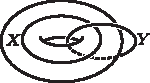
\includegraphics[scale=1]{AnnulusOption.pdf}}}}}
\AnnulusOption
\quad \quad \leftrightarrow \quad \quad 
\AddDatTorus{\FubeXXXA}{X}{Y}\quad \quad \quad X,Y \in\{ B, N \}
\end{align}
\caption{\label{TorusNotation} 
To go from the annulus to the torus we identify the inner and outer circles, and label the different spin structures by $X$ and $Y$ for the longitudinal and meridional cycles on the torus, respectively.
}
\end{figure}




If there was no interplay between a chosen spin structure and the string-net pictures drawn on the torus, 
and if the fermion parity of a ground state is fixed by the spin structure 
and the string-net picture drawn on the torus, we would expect $|H_1(T^2;\zt)|=4$ 
degenerate ground states 
for each choice of spin structure, since the $\beta$ lines obey $\zt$ fusion rules. 
We will see that naive guess is incorrect: instead, for each spin structure, 
one of the four putative states is a null vector, meaning that there is only a 
3-dimensional groundstate for each choice spin structure.

We will first use elementary arguments to find a spanning set for each of the four spin tori.
Later, using more sophisticated techniques, we will prove that these spanning sets are in fact bases.

Since $\beta$ lines obey $\zz/2$ fusion rules (see \ref{C2_data_table}), it is easy to see that any string net on a spin torus
is a linear combination of the following seven diagrams:
\be \label{seven_tubes} \Fubex{\FubeXXXA}{},\;  \Fubex{\FubesXsA}{},\;     \Fubex{\FubesdXsA}{},\; 
\Fubex{\FubeXssA}{},\; \Fubex{\FubeXsdsA}{},\; \Fubex{\FubessXA}{}, \; \Fubex{\FubessdXA}{}.
\ee
Indeed, using \eqref{Fmove} and the ability to remove topologically trivial $\beta$ loops, 
we can transform the $\beta$ loops into a standard representative of their
$\zz/2$ homology class.
The resulting loop will be decorated by some number of fermionic dots; using dot cancellation we can assume that the
loop will contain either 0 or 1 dot.
The seven diagrams listed above are the only independent diagrams that remain after applying these relations. 


However, for a given spin structure, some of the diagrams in \eqref{seven_tubes} will be zero.
To determine which of the diagrams are zero, we use the following three obervations:
\begin{enumerate}
	\item If one of the non-trivial cycles of the torus has an antiperiodic spin structure, then any odd diagram is zero.
	This is because we can translate the entire string net in the direction of the antiperiodic cycle.
	When we arrive back at our starting point, we have picked up a factor of $-1$ from the antiperiodicity.
	Thus odd diagrams are equal to $-1$ times themselves and are therefore zero.
	In particular, the three odd diagrams of \eqref{seven_tubes} are zero in the $BB$, $BN$ and $NB$ spin structures.
	\item If a diagram contains a $\beta$ loop without a dot (even fermion parity), and if that loop inherits the periodic spin structure,
	then the diagram is zero.
	To see this, we create two dots on the loop, slide one around the loop, and then cancel the dots again.
	Because of the Koszul sign, we see that the diagram is equal to $-1$ times itself.
	(If the spin structure along the cycle were antiperiodic, there would be an additional sign to cancel the Koszul sign.)
	In particular, in the $NN$ spin structure all three of the even $\beta$ loops are zero.
	For the $BB$, $BN$ and $NB$ spin structures, exactly one of the three even $\beta$ loops fails this test and is zero.
	\item Finally, the empty diagram with $NN$ spin structure is zero. To show this, 
	we first create a topologically trivial circular $\beta$ loop. We then wrap it around the tube and fuse it 
	with itself to get the sum of two diagrams with parallel $\beta$ loops wrapping around the tube, one of 
	which has no fermion dots (the even channel of $\beta\tp \beta$) and one which has one dot on each $
	\beta$ loop (the odd fusion channel of $\beta\tp\beta$). 
	The diagram corresponding to the even fusion channel 
	is zero by observation 2 above, while the diagram with two odd loops is zero by an argument similar to observation 2: we slide one of the loops in the direction
	orthogonal to itself and pick up a Koszul sign, showing that the diagram must be zero.
\end{enumerate}

Figure \ref{TorusBasisC2} shows the remaining non-zero diagrams for each spin structure.
It is easy to see that these diagrams are linearly independent if they are non-zero, but we have not yet proved that they are in fact non-zero.
To do this, we will employ a fancier argument relating a basis of the torus Hilbert space to minimal idempotents of the tube category.

Let $\tube^B$ denote the bounding tube category and $\tube^N$ denote the non-bounding tube category.
We can make use of the following results, which we prove in a more general context in Section \ref{torus_basis_theorem}:
The ground state spaces of the ${BB}, {NB},$ and ${BN}$ tori are purely even, with an orthogonal basis given by closed-up minimal idempotents of $\tube^B$.
Additionally, the ground state space of the $NN$ torus is isomorphic to $\cc^{p|q}$, where $p$ is the number of m-type idempotents of $\tube^N$
and $q$ is the number of q-type idempotents of $\tube^N$.
An orthogonal basis is given by (representatives of) the minimal m-type idempotents of $\tube^N$,
union $\{\cl(\gamma_j)\}$,
where $\gamma_j$ runs through a set of representatives of odd endomorphisms of the minimal q-type idempotents of $\tube^N$.
We use $\cl$ to denote the closure of an annular diagram on the torus.

For the $C_2$ theory, we have shown that $\tube^B$ has three m-type minimal idempotents, 
and $\tube^N$ has three q-type minimal idempotents.
Letting $A(T^2_{JK})$ denote the Hilbert space on the torus with $JK$ spin structure, 
it follows that $A(T^2_{BB}) \cong A(T^2_{NB}) \cong A(T^2_{BN}) \cong \cc^{3|0}$ and
$A(T^2_{NN}) \cong \cc^{0|3}$,
and so the diagrams of Figure \ref{TorusBasisC2} must indeed all be non-zero.




\begin{figure}
  \centering
    \begin{align}
\nonumber
\begin{array}{ l l l l }
\multicolumn{1}{c}{A(T^2_{XY})} &{\quad \quad \quad}& \multicolumn{1}{c}{\text{explicit basis}} & \\ \cline{1-1}\cline{3-3} && &\\
A(T^2_{BB}) \cong \mathbb{C}^{3|0} & & \AddDatTorus{\FubeXXXA}{B}{B} , \; \AddDatTorus{\FubesXsA}{B}{B}, \;  \AddDatTorus{\FubeXssA}{B}{B} &\\   
&&&\\
A(T^2_{BN}) \cong \mathbb{C}^{3|0} & & \AddDatTorus{\FubeXXXA}{B}{N} , \; \AddDatTorus{\FubesXsA}{B}{N}, \;  \AddDatTorus{\FubessXA}{B}{N} &\\  
&&&\\
A(T^2_{NB}) \cong \mathbb{C}^{3|0} & & \AddDatTorus{\FubeXXXA}{N}{B} , \; \AddDatTorus{\FubeXssA}{N}{B}, \;  \AddDatTorus{\FubessXA}{N}{B} &  \\
&&&\\
A(T^2_{NN}) \cong \mathbb{C}^{0|3} & & \AddDatTorus{\FubesdXsA}{N}{N} , \; \AddDatTorus{\FubeXsdsA}{N}{N}, \;  \AddDatTorus{\FubessdXA}{N}{N} &\\  
&&&\\ 
\end{array}
\end{align}
\caption{\label{TorusBasisC2} The ground states on the four different spin tori. 
Notice that the non-bounding torus (with $NN$ spin structure) has only odd fermion parity ground states.}
\end{figure}



For future reference we also tabulate the change of basis between the ground-state tori in Figure \ref{TorusBasisC2} 
and the closed-up primitive idempotents.
To form string-net pictures drawn on tori from the idempotents, 
we close up the idempotents along the longitudinal direction by identifying the inner boundary 
of the annulus on which the idempotent lives with the outer boundary, 
specifying a choice of spin structure along the newly made cycle. 
We then express the result as a linear combination of the tori in Figure \ref{TorusBasisC2}.
For simplicity of notation, we will define 
\begin{align}
e=\; {\FubeXXXA} \quad h = \;{\FubesXsA}  \quad v =\; {\FubeXssA} \quad t = \; {\FubessXA}
\end{align}
and append subscripts to denote a particular spin structure. 
We will also use an overscript $\bullet$
if we are closing up an odd endomorphism rather than the idempotent itself.
For example,
\begin{align}
h_{NB}= \; \AddDatTorus{\FubesXsA}{N}{B} \quad \quad \text{and} \quad \quad \overset{\bullet}{t}_{NN} = \AddDatTorus{\FubessdXA}{N}{N} \; .
\end{align}
We can then compute the change of basis shown in Figure \ref{C2Change_of_Basis}.
\begin{figure}
  \centering
\begin{align}
\nonumber
\left( \begin{matrix}
m_\unit \\
m_\sigma^+\\
m_\psi \\
\end{matrix} \right)_{BB} 
&= \frac{1}{2}\left( \begin{matrix}
1&1/d&0\\
0&0&1\\
1&-1/d&0\\
\end{matrix} \right)
\left( \begin{matrix}
e\\
h\\
v\\
\end{matrix} \right)_{BB}
\quad \quad \quad
\left( \begin{matrix}
m_\unit \\
m_\sigma^+\\
m_\psi \\
\end{matrix} \right)_{BN} 
= \frac{1}{2}\left( \begin{matrix}
1&1/d&0\\
0&0&A^3\\
1&-1/d&0\\
\end{matrix} \right)
\left( \begin{matrix}
e\\
h\\
t\\
\end{matrix} \right)_{BN}\\
\nonumber
\left( \begin{matrix}
q_\unit \\
q_\sigma\\
q_\psi \\
\end{matrix} \right)_{NB} 
&= \frac{1}{2}\left( \begin{matrix}
0&1&A^5\\
2&0&0\\
0&1&-A^5\\
\end{matrix} \right)
\left( \begin{matrix}
e\\
v\\
t\\
\end{matrix} \right)_{NB}
\quad \quad \quad
\left( \begin{matrix}
\overset{\bullet}{q}_\unit \\
\overset{\bullet}{q}_\sigma\\
\overset{\bullet}{q}_\psi \\
\end{matrix} \right)_{NN} 
= \frac{1}{2}\left( \begin{matrix}
0&A^6&-A^{3}\\
\sqrt{2}&0&0\\
0&A^6&A^{3}\\
\end{matrix} \right)
\left( \begin{matrix}
\overset{\bullet}{h}\\
\overset{\bullet}{v}\\
\overset{\bullet}{t}\\
\end{matrix} \right)_{NN}
\end{align}
\caption{Change of basis between the quasiparticle (idempotent) basis given in Table \eqref{CTwoParticles} 
and the topological bases in Figure \eqref{TorusBasisC2} for the torus.
These are simply given by expressing the idempotents in the topological bases. 
Note that the odd torus has a sign ambiguity on each of the of the idempotents. 
We can require that $(\overset{\bullet}{q})^2 = q$, but that leaves $\overset{\bullet}{q}$ ambiguous up to a $\pm$ sign. 
This ambiguity can lead to different $S$ matrices, see \eqref{NNSmatrix} and surrounding text for more details.}
\label{C2Change_of_Basis}
\end{figure}


%%%%%%%%%%%%%%%%%%%%%%%%%%%%%
\subsubsection{The modular $S$ and $T$ matrices} \label{C2_modular_mats}
%%%%%%%%%%%%%%%%%%%%%%%%%%%%%

\begin{figure} 
\newcommand{\Space}{\; \; \; \; \; \; }
\newcommand{\Spacep}{ \; \; \; \mathop{\vphantom{\int}} \; \; \;    } 
\begin{align}
\nonumber
\xymatrix@!0 @M=1mm @R=7mm @C=30mm{
\AddDatTorus{\FubeXXXA}{B}{B}\ar @`{p+(-28.28,7.07),p+(-7.07,28.28)}^{S}  \ar@<1ex>[r]^T  & \AddDatTorus{\FubeXXXA}{B}{N} \ar@<1ex>[l]^T   \ar@<1ex>[r]^S&  \AddDatTorus{\FubeXXXA}{N}{B}  \ar@<1ex>[l]^S  \ar @`{p+(7.07,28.28),p+(28.28,7.07)}^{T } &\AddDatTorus{\FubeXXXA}{N}{N}  \ar @`{p+(7.07,28.28),p+(28.28,7.07)}^{S,T } 
}
\end{align} \nonumber
\caption{\label{spin_str_mapping_class_group}The action of the mapping class group on the four spin tori. 
}
\end{figure}

In this section, we will compute the representation of the modular $S$ and $T$ matrices in the $C_2$ theory, which together generate the modular groupoid. 
The modular $S$-matrix acts on states on the torus by interchanging the meridional and longitudinal cycles 
of the torus.
If we draw the torus as a square with opposite sides identified, then $S$ acts by rotating the square by $\pi/2$ clockwise. 
The modular $T$ matrix represents the action of the Dehn twist on the torus, 
which corresponds to cutting the torus along a meridional cycle, 
twisting the boundary conditions at the cut by $2\pi$ relative to one another, and gluing the torus back together.
In terms the annular pictures we have been drawing of the tubes, the twist is accomplished by 
twisting the inner boundary of the annulus by $2\pi$ counterclockwise relative to the outer boundary. 

Importantly, the $S$ and $T$ modular transformations do {\it not} always preserve the spin structure of the torus they act on. 
Figure \ref{spin_str_mapping_class_group} shows how the different possible spin structures are permuted under $S$ and $T$. 
Since $T$ does not preserve the spin structures, it cannot have well-defined eigenstates with a definite spin structure,
meaning that it will not be diagonal in the idempotent (quasiparticle) basis. 
This means that the topological spins of bounding (non-vortex) quasiparticles, defined as their eigenvalues under $T$, will not be well-defined.
In contrast with $T$, the action of $T^2$ preserves spin structures, and so we are still able to associate 
definite $T^2$ 
eigenvalues to the quasiparticles in the theory.
Putting aside the issue of spin structures, the twist of an idempotent (defined as the phase acquired when performing a $2\pi$ twist on the tubes in a given idempotent) 
is in general only defined 
up to a $\pm$ sign (which has been discussed in e.g. \cite{cano2014,bruillard2017,gu2014}).
More precisely, the twist of a given simple object in the tube category is ambiguous across the isomorphism 
class of that object. 
Indeed, we will see that the twists of the two idempotents in the $m_\sigma$ isomorphism class (namely $m_\sigma^+$ and 
$m_\sigma^-$) have twists that differ by a factor of $-1$. 

We now proceed to examine the action of the $S$ and $T$ modular transformations on the four spin tori which compose 
the 12-dimensional space listed in Figure \ref{TorusBasisC2}.
Although the calculations are most easily performed in the topological basis in Figure \ref{TorusBasisC2}, 
it is more natural to analyze the resulting transformations in the idempotent basis given in Table \ref{CTwoParticles}. 
As mentioned earlier, the basis vectors in the idempotent basis are constructed by taking the idempotents associated with the 
quasiparticles identified in the previous section and closing them up (with different choices of spin structure) 
along the longitudinal direction. 
The change of basis between the topological and idempotent bases are written explicitly in Figure \ref{C2Change_of_Basis}. 


We'll start with the $BB$ spin structure, which is preserved under the action of $S$. 
In the topological basis $(e,v,h)^T$ we find
\begin{align}
\left( \begin{matrix}
e\\
v\\
h\\
\end{matrix} \right)_{BB} 
\xrightarrow{S^{BB \rightarrow BB}} & \left( \begin{matrix}
1&0&0\\
0&0&1\\
0&1&0\\
\end{matrix} \right)
\left( \begin{matrix}
e\\
v\\
h\\
\end{matrix} \right)_{BB}.
\end{align}
To transform $S^{BB\rightarrow BB}$ into the quasiparticle basis we use Figure \ref{C2Change_of_Basis}.
After the change of basis we find the familiar matrix
\begin{align}
\left( \begin{matrix}
m_\unit\\
m_\sigma^+\\
m_\psi \\
\end{matrix} \right)_{BB} 
\xrightarrow{S^{BB \rightarrow BB}} &\frac{1}{2} \left( \begin{matrix}
1&d&1\\
d&0&-d\\
1&-d&1\\
\end{matrix} \right)
\left( \begin{matrix}
m_\unit\\
m_\sigma^+\\
m_\psi \\
\end{matrix} \right)_{BB}
\end{align}
which is identical to the $S$-matrix for the Ising TQFT. 

Now for the $BN$ and $NB$ spin structures.
These are interchanged by the $S$-matrix, as indicated in Figure \ref{spin_str_mapping_class_group}.
In the idempotent bases these induce transformations between the non-vortex and vortex quasi-particles.
We obtain 
\begin{align}
\left( \begin{matrix}
e\\
h\\
t\\
\end{matrix} \right)_{BN} 
\xrightarrow{S^{BN \rightarrow NB}} & \left( \begin{matrix}
1&0&0\\
0&1&0\\
0&0&A^{10}\\
\end{matrix} \right)
\left( \begin{matrix}
e\\
v\\
t\\
\end{matrix} \right)_{NB}
\quad \text{and} \quad 
\left( \begin{matrix}
e\\
v\\
t\\
\end{matrix} \right)_{NB} 
\xrightarrow{S^{NB \rightarrow BN}} & \left( \begin{matrix}
1&0&0\\
0&1&0\\
0&0&A^{6}\\
\end{matrix} \right)
\left( \begin{matrix}
e\\
h\\
t\\
\end{matrix} \right)_{BN}.
\end{align}
Notice that if we compose both transformations we get the identity. 
These can each be transformed into the idempotent bases using \eqref{C2Change_of_Basis}, 
where one finds,
\begin{align}
\left( \begin{matrix}
m_\unit\\
m_\sigma^+\\
m_\psi\\
\end{matrix} \right)_{BN} 
\xrightarrow{S^{BN \rightarrow NB}} &\frac{1}{2} \left( \begin{matrix}
1&d&1\\
-d&0&d\\ 
-1&d&-1\\
\end{matrix} \right)
\left( \begin{matrix}
\hat{q}_\unit\\
\hat{q}_\sigma^+\\
\hat{q}_\psi\\
\end{matrix} \right)_{NB}
\end{align}
and
\begin{align}
\label{closing_q_type_C2}
\left( \begin{matrix}
\hat{q}_\unit\\
\hat{q}_\sigma^+\\
\hat{q}_\psi\\
\end{matrix} \right)_{NB} 
\xrightarrow{S^{NB \rightarrow BN}} & \frac{1}{2}\left( \begin{matrix}
1&-d&-1\\ 
d&0&d\\
1&d&-1\\
\end{matrix} \right)
\left( \begin{matrix}
m_\unit\\
m_\sigma^+\\
m_\psi\\
\end{matrix} \right)_{BN}.
\end{align}
In order to make the matrix unitary, we have defined $\hat{q} = q/\sqrt{2}$ so that each $\hat{q}$ idempotent has unit norm (how to compute the norms of idempotents will be discussed in Section \ref{traces_and_innerproducts}). 
To collect the results we've arrived at so far, we define
\begin{align}
{\bf M} = [ m_\unit \;  m_\sigma^+\;  m_\psi]^T \qquad \widehat{{\bf Q} }= [\hat{q}_\unit \; \hat{q}_\sigma \; \hat{q}_\psi ]^T
\end{align}
Then we have,
\begin{align}
\left( \begin{matrix}
{\bf M}_{BN}\\
\widehat{{\bf Q} }_{NB}\\
{\bf M}_{BB}\\
\end{matrix} \right)
\xrightarrow{\;\; S \; \; } & \left( \begin{matrix}
&S^{BN \rightarrow NB}&\\
S^{NB \rightarrow BN}&&\\
&&S^{BB \rightarrow BB}\\
\end{matrix} \right)
\left( \begin{matrix}
{\bf M}_{BN}\\
\widehat{{\bf Q} }_{NB}\\
{\bf M}_{BB}\\
\end{matrix} \right).
\end{align}

Similarly we can compute the modular $T$-matrix, the action of which twists the inner boundary of an annulus by an angle of $2\pi$ counterclockwise with respect to its outer boundary. 
This definition ensures that the $T$-matrix acts as the identity on tubes with no charge line 
(i.e. with no strings ending on their inner annular boundaries).
Within each spin structure sector the $T$-matrix is diagonal in the idempotent basis. 
We can read off the structure of the $T$-matrix with the help of Figure \ref{spin_str_mapping_class_group} to find
\begin{align}
\left( \begin{matrix}
{\bf M}_{BN}\\
\widehat{{\bf Q} }_{NB}\\
{\bf M}_{BB}\\
\end{matrix} \right)
\xrightarrow{\;\; T \; \; } & \left( \begin{matrix}
&&T^{BN \rightarrow BB}\\
&T^{NB \rightarrow NB}&\\
T^{BB \rightarrow BN}&&\\
\end{matrix} \right)
\left( \begin{matrix}
{\bf M}_{BN}\\
\widehat{{\bf Q} }_{NB}\\
{\bf M}_{BB}\\
\end{matrix} \right).
\end{align}
With 
\begin{align}
T^{BN \rightarrow BB} =  & \left( \begin{matrix}
1&&\\
&A^3&\\
&&1\\
\end{matrix} \right)
\quad 
T^{NB \rightarrow NB}=  & \left( \begin{matrix}
A^5&&\\
&1&\\
&&-A^5\\
\end{matrix} \right)
\quad 
T^{BB \rightarrow BN}=  & \left( \begin{matrix}
1&&\\
&A^3&\\
&&1\\
\end{matrix} \right)
\end{align}
One can check that the usual modular group relation $(ST)^3 = \unit$ holds as expected. 


More interesting is the $NN$ torus, whose spin structure is preserved under both $S$ and $T$. 
This has been investigated before in \cite{ware2016}, and our results agree with theirs in this case. 
According to Figure \ref{TorusBasisC2}, the Hilbert space is spanned by $\overset{\bullet}{h}$, $\overset{\bullet}{v}$, and $\overset{\bullet}{t}$,
where as before the $\bullet$ means that the associated tubes have odd fermion parity.
In the topological basis, we obtain
\begin{align}
\left( \begin{matrix}
\overset{\bullet}{h}\\
\overset{\bullet}{v}\\
\overset{\bullet}{t}\\
\end{matrix} \right)_{NN} 
\xrightarrow{S^{NN \rightarrow NN}} & \left( \begin{matrix}
0&1&0\\
 A^4&0&0\\
0&0&A^{10}\\
\end{matrix} \right)
\left( \begin{matrix}
\overset{\bullet}{h}\\
\overset{\bullet}{v}\\
\overset{\bullet}{t}\\
\end{matrix} \right)_{NN}
\end{align}
Now we need to transform into the idempotent (quasiparticle) basis. 
With the choice of basis in Figure \ref{C2Change_of_Basis} we find
\begin{align}
\left( \begin{matrix}
\overset{\bullet}{q}_\unit\\
\overset{\bullet}{q}_\sigma\\
\overset{\bullet}{q}_\psi\\
\end{matrix} \right)_{NN} 
\xrightarrow{S^{NN \rightarrow NN}} &\frac{-A^2}{2} \left( \begin{matrix}
1& d&-1\\
d&0&d\\
-1& d&1\\
\end{matrix} \right)
\left( \begin{matrix}
\overset{\bullet}{q}_\unit\\
\overset{\bullet}{q}_\sigma\\
\overset{\bullet}{q}_\psi\\
\end{matrix} \right)_{NN}.
\label{NNSmatrix}
\end{align}
Note that the requirement $\overset{\bullet}{q}^2 =q$ only determines $\overset{\bullet}{q}$ up to a $\pm$ sign. 
Consequently the off-diagonal matrix elements $(S^{NN \ra NN})_{ij}$ between q-type idempotents are only determined up to a sign 
(indeed, sending $\overset{\bullet}{q}_j \ra s_j \overset{\bullet}{q}_j$, $s_j =\pm1$ conjugates the S-matrix by a diagonal matrix of $\pm1$'s).
Similarly, we can compute the modular $T$-matrix, 
\begin{align}
\left( \begin{matrix}
\overset{\bullet}{q}_\unit\\
\overset{\bullet}{q}_\sigma\\
\overset{\bullet}{q}_\psi\\
\end{matrix} \right)_{NN} 
\xrightarrow{T^{NN \rightarrow NN}} &\left( \begin{matrix}
A^5& &\\
&1&\\
&&-A^5\\
\end{matrix} \right)
\left( \begin{matrix}
\overset{\bullet}{q}_\unit\\
\overset{\bullet}{q}_\sigma\\
\overset{\bullet}{q}_\psi\\
\end{matrix} \right)_{NN}
\end{align}
One can check that we have the modular relations
\begin{align}
 (S^{NN\ra NN}T^{NN\ra NN})^3 = (S^{NN \ra NN})^4= A^{8}\text{id} = -\text{id}
\end{align}
The minus sign comes from the fact that acting by $S^4$ or $(ST)^3$ performs a $2\pi$ rotation 
of the fermion framing, resulting in a phase of $-1$, since all states on the $NN$ torus have odd fermion parity. 
For general theories, these relations become $(ST)^3=S^4=(-1)^F$, where $(-1)^F$ is the fermion 
parity operator.
See Sections \ref{SO36ModularTransformations} and \ref{E6S_matrix_section} for examples of this more general scenario. 


\medskip

Collecting these results, we can now write down the complete modular $S$ and $T$ matrices in the $C_2$ theory, 
which act across all spin structures. 
In the quasiparticle 
basis $[(m_\unit,m_\sigma^+,m_\psi)_{BB},(m_\unit,m_\sigma^+,m_\psi)_{BN},(q_\unit,q_\sigma,q_\psi)_{NB},(\overset{\bullet}{q}_\unit,\overset{\bullet}{q}_\sigma,\overset{\bullet}{q}_\psi)_{NN}]^T$, 
we have
\be \label{modularS}
S = \frac{1}{2}\begin{pmatrix} 1 & d & 1 &			&&&			&&&			&& \\ 
					      d & 0 &-d &			&&&			&&&			&&\\
					      1&-d&1 & 			&&&			&&&			&&\\
						&&&				&&&			1&d&1&		&& \\
						&&&				&&&			-d&0&d&		&&\\ 
						&&&				&&&			-1&d&-1&		&&\\
						&&&				1&-d&-1&		&&&			&&\\ 
						&&&				d&0&d&		&&&			&&\\
						&&&				1&d&-1&		&&&			&&\\ 
						&&&				&&&			&&&			-A^{2} & -A^{2}d & A^{2}\\
						&&&				&&&			&&&			-A^{2}d & 0 & -A^{2}d \\ 
						&&&				&&&			&&&			A^{2} & -A^{2}d & -A^{-2} \end{pmatrix}\ee		
where we have only listed the non-zero entries. 
$S$ has two different direct-sum decompositions. First, essentially by construction, 
it splits into a direct sum over blocks according to spin structures 
under the $S$ modular transformation. 
Additionally, we have $S = S_{even} \oplus S_{odd}$, where $S_{odd}$ is the $S$-matrix 
acting on ground states with odd fermion parity.
This decomposition is always possible, but it will not always match a decomposition based 
on spin structures. 
That is, while $S_{odd} = S^{NN\ra NN}$ in this theory, spin structure blocks of $S^{NN\ra NN}$ 
will not have a definite fermion parity in general; see Sections \ref{so36} and \ref{halfesix} for examples. 
Also note that $S^4 = \unit_{9\times9}\oplus(-\unit_{3\times3})$ in accordance with $S = S_{even} \oplus S_{odd}$ and $S^4=(-1)^F\unit$. 

Now for the $T$-matrix. 
In the same quasiparticle basis as before, the $T$-matrix is
\be 
T = \begin{pmatrix}   			&&&				1&0&0&		&&&			&& \\ 
					        &&&				0&A^3&0&	&&&			&&\\
					        &&& 				0&0&1&		&&&			&&\\
						1&0&0&			&&&			&&&			&& \\
						0&A^3&0&		&&&			&&&			&&\\
						0&0&1&			&&&			&&&			&&\\
						&&&				&&&			A^{5}&0&0&	&&\\
						&&&				&&&			0&1&0&		&&\\
						&&&				&&&			0&0&-A^{5}&	&&\\
						&&&				&&&			&&&			A^{5}&0&0\\
						&&&				&&&			&&&			0&1&0 \\ 
						&&&				&&&			&&&			0&0&-A^{5} \end{pmatrix}\ee	
The $T$-matrix is not completely diagonalized in the idempotent basis, since it acts nontrivially on the spin structures (although it is diagonalized within each spin structure block). 

%%%%%%%%%%%%%%%